\documentclass{article}
\usepackage[czech]{babel}
\usepackage[utf8]{inputenc}   % pro unicode UTF-8
\usepackage{graphicx}   % pro unicode UTF-8

\begin{document}

\title{Business Process Diagrams}

This document describes main workflow and business processes related to the
Deska Database, part of the Tool for Central Administration of a Grid Site.
All the operations can be described using a form of the single flow diagram.


\section{Business Process}

\subsection{Workflow}
This part describes the state changes involved when the only actor,
Administrator, performs various changes.  All the operations which involve the
database can be described using the following flow diagram.

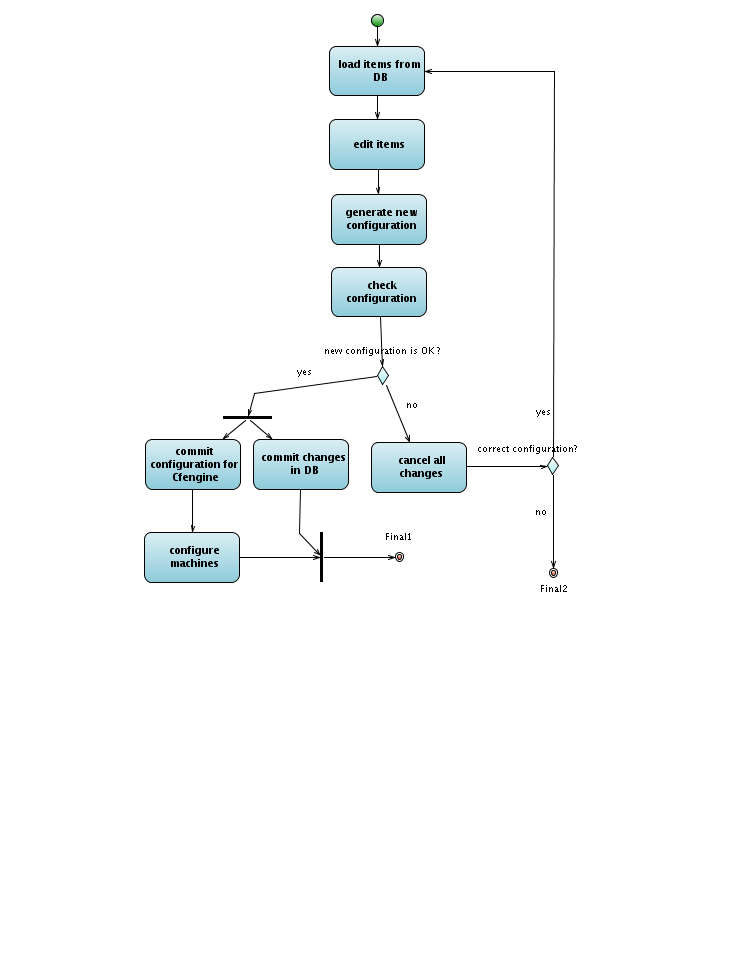
\includegraphics[height=14cm]{business_process.png}

\subsubsection{Load items form DB}
The purpose of this state is to guarantee that the system is working with fresh
data.

Scenario:
\begin{itemize}
    \item{A connection to the database is established}
    \item{Internal data structures are fetched form the database}
    \item{System moves to the {\em Edit items} state}
\end{itemize}

\subsubsection{Edit items}
The Administrator performs the desired changes using her favorite interface

Scenario:
\begin{itemize}
    \item{A list of machines is presented to the Administrator}
    \item{Administrator edits the data}
    \item{System moves to {\em Generate new configuration} state}
\end{itemize}

\subsubsection{Generate new configuration}
A tool which processes the new snapshot of the database is invoked and new
generated configuration prepared

Scenario:
\begin{itemize}
    \item{The new state of the database (a snapshot) is stored and the snapshot
        gets traversed by the system}
    \item{System generates new generated configuration based on the data from
        the snapshot}
    \item{The newly prepared generated configuration is added to the snapshot
        with the new database state}
    \item{From now on, both sets of changes, that is new database state and
        related newly generated configuration, are closely coupled together and
        must not be touched individually}
    \item{System moves to {\em Check configuration} state}
\end{itemize}

\subsubsection{Check configuration}
The administrator reviews the new snapshot for correctness

Scenario:
\begin{itemize}
    \item{New database state {\bf and} the newly generated configuration is
        provided for the Administrator for review}
    \item{The Administrator checks both changesets for correctness, especially
        whether both changes corresponds properly}
    \item{In case of failure, system moves to the {\em Rollback} state}
    \item{In success case, system moves to the {\em Commit} phase}
\end{itemize}

\subsubsection{Rollback}
All changes are being reverted

Scenario:
\begin{itemize}
    \item{The whole snapshot, both in the database and in the generated
        configuration, is thrown away}
    \item{If the Administrator wants to fix changes, system moves to the initial
        state}
    \item{If the Administrator does not want to try to perform changes again,
        the system moves to the {\em Final2} state}
\end{itemize}

\subsubsection{Commit}
New changes are committed

Scenario:
\begin{itemize}
    \item{If the database and configuration files are stored in the same
        backend, both are committed in the same step and in an atomic manner}
    \item{Otherwise, the DB gets committed and new configuration files are
        pushed to the repository}
    \item{System moves to the {\em Final1} state}
\end{itemize}

\subsubsection{Configuring machines}
The newly generated configuration files are picked up by the configuration
distribution system

Scenario:
\begin{itemize}
    \item{An already deployed system like Cfengine pushes the newly generated
        configuration files to all machine nodes}
    \item{Changes get picked up by the services running on machines}
    \item{System moves to an initial state}
\end{itemize}


\subsubsection{Delete machine}
Delete machine from the grid site.

Scenario:
\begin{itemize}
\item{Administrator chooses, that he wants to delete existing machine}
\item{Include (select machine)}
\item{Include (confirm changes)}
\end{itemize}

\subsubsection{View configuration}
View configuration of machine from the grid site.

Scenario:
\begin{itemize}
\item{Administrator chooses, that he wants to see configuration of existing machine}
\item{Include (select machine)}
\item{System generates and view complete report from current configuration of the machine}
\end{itemize}

\section{Project Glossary}

Refer Tool for Central Administration of a Grid Site document.

\end{document}
